\chapter{Marketing startegies}\label{ch:B}

\section{Social Media Marketing (SMM) in Donor project}
SMM currently transcends all boundaries and continues to play an important role in human life, all people have social networks where they spend most of their time \cite{macarthy}. They provide a single platform for companies to keep in touch with their customers and offer themselves or their product \cite{macarthy}.
\par
The number of social networks continues to grow in the world, and each of them has integration that helps to promote a particular business company in which the users themselves are interested. Therefore, developing companies strive for advertising promotions and SMM itself. Someone may say that this is the future prosperity of companies and we agreed with this statement and decided to use this in our project.
\par
Taking such steps as creating posts in the SMM format, we are preparing a skeleton of what we are and showing a novelty for some people. So by building the brand, preparing the website, we went to build a community around the brand to increase our loyal customer base.(see Figure \ref{fig:storyscreenshot})
\begin{figure}[h]
    \centering
    
\includegraphics[scale=0.7]{figures/6.jpeg}
    \caption{Instagram Story screenshot}
    \label{fig:storyscreenshot}
\end{figure}

\par
Before all this, what was said above, having familiarized ourselves with some sources, we came across advice to analyze the market in demand and need. We started this with the demand step. First of all Instagram stories went into action with a survey and helped to analyze the market as we said earlier. 

\section{Target and promotions online}

\par
After analyzing such types of stories in Instagram, this gave us several dozen responses, people were ready to help and there were a lot of donors. A lot of people had a feedback on such publication, but among them there were people who wanted to help but did not know how it all works, people who do not have enough information about donation. Thanks to this, we concluded that this project has a demand, so we decided to move on by launching a target page. 
\par
Targeting is a good option for a promotion, especially it is good for the 'Donor project', because it is an online platform and most of the user will definitely come from social media.
To target our potential donors, we created a new account on Instagram and began to promote it through stories, posts of friends, and then completely through the target. (see Figure \ref{fig:igaccount})
\begin{figure}[h]
    \centering
    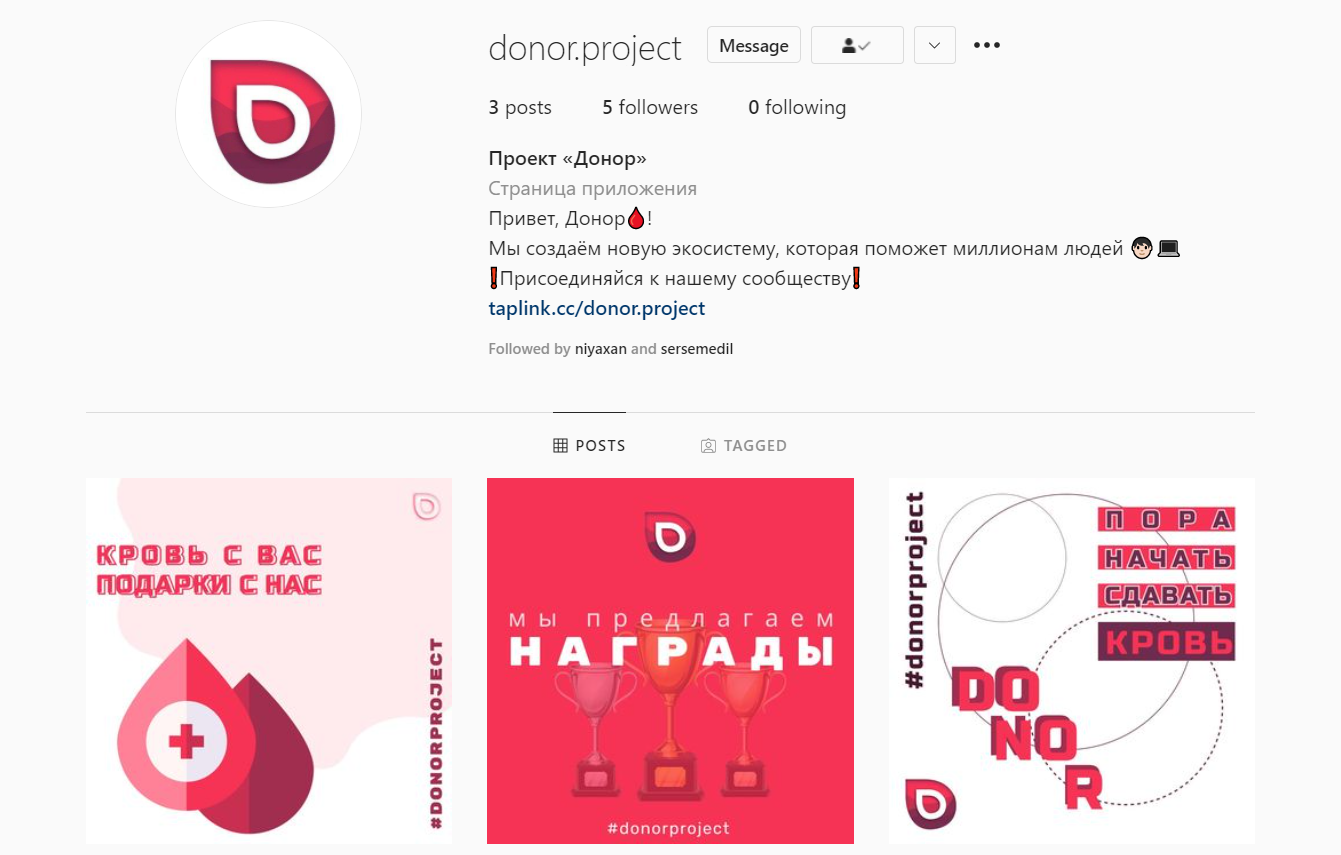
\includegraphics[scale=0.25]{figures/7.png}
    \caption{Instagram Profile of Donor project}
    \label{fig:igaccount}
\end{figure}
\par
To begin with, we went to the Facebook ads manager and set up everything that was needed for promotion. We posted a target, it was moderated and started working. Thus, they called and explained enlightened people in our project, indicating a link to our account intended for redirecting to a website. In our humble way, doing this business, that is, enlightenment, we think that we are helping to make this world a better place.
The Instagram account will also be entered by us. Our main logo was added to the branding of the account, which we put in the avatar. Also, to explain what we are, we threw a few posts with an explanation. After working in Figma, we made illustrations for posts.

\section{Award system and Integration}
Awards and privileges are a collection system for donating blood. On our site there is a separate page with all the possible bonuses that you can get and the prices next to it. Though the prices are indicated not in money, but in the campaigns of the blood donation. Prices are indicated in the site accumulation system and for each donation of blood you are credited with a certain number of bonuses. 
\par
Thus, having some points on your intra-site balance, you can purchase the bonuses that are available and provided by our program. Everyone can get acquainted with this on the page. If there are enough points on your account, you are asked to purchase one of the services to choose from. You buy some of the services if everything is correct and approved for you and you have a balance suitable for success. You can see more details on how many points you need under each bonus card that is provided on the website.
(see Figure \ref{fig:bonuses})

\begin{figure}[h]
    \centering
    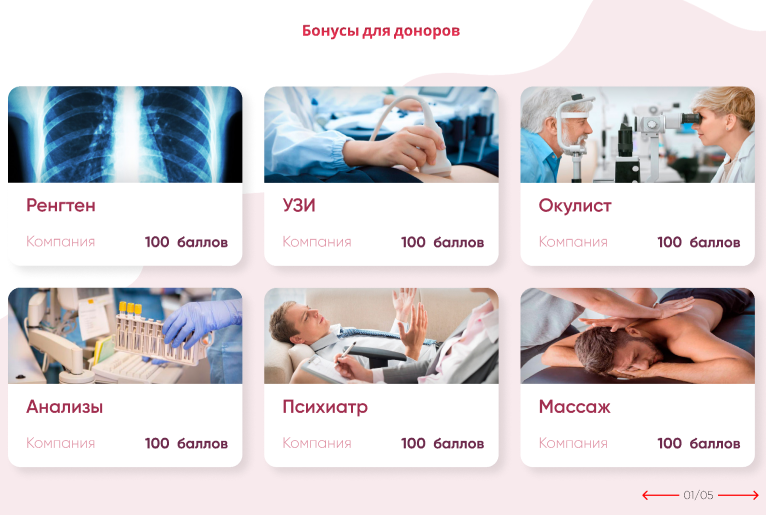
\includegraphics[scale=0.5]{figures/8.png}
    \caption{Bonus page of Donor project}
    \label{fig:bonuses}
\end{figure}
\par
As the statistics of visits has shown, this will be useful not only for our clients, but also for medical institutions. The donor donates blood by receiving bonuses, he goes to receive bonuses by choosing a medical institution. Receives a bonus, satisfaction, and on a subconscious level, the donor wants to return to the place where he received the bonus. 
\par
That is, we want to say that an ordinary user gets a profit from donating blood in exchange for receiving bonuses, and on the other hand, these hospitals where they provide services find new customers through our system. Thus, the two sides satisfy human and monetary needs.

\section{Badges of activity}
The main important thing of an online platform is to provide user ability of entertainment \cite{macarthy}. As we don't promote ourselves as an official presence such as news portal or governmental project, the idea of awarding developed through the process of working on the project. 
\par
System of awarding people with badges creates strong connection between simple user \cite{eyal}. As the researches show, people want to belong to a community and share ideas and thoughts that correlate with their own mind. Badge system was developed in order to prioritize layer of donors, so that new users will have a motivation not only to donate blood, but also receive some kind of appreciation of them in our system.
\par
There are special achievements for users, just like in games. These are not bonuses, this is a separate page on the site where various achievements are displayed and in order to complete them a user needs to complete blood donation history, depending on the number of blood donations and time. To open any achievement, user needs to follow your instructions in the description of the achievements.
\par
This will not only be interesting a user itself, but it will attract his friends and relatives, because, as the research shows, people are always trying to compete in different possible areas \cite{eyal}. And such competition as blood donation and enormous help to people in need is the best application.
(see Figure \ref{fig:achievements})

\begin{figure}[h]
    \centering
    
\includegraphics[scale=0.4]{figures/9.png}
    \caption{Achievements in Donor project}
    \label{fig:achievements}
\end{figure}